\section{实验结果及分析}
\subsection{ALU验证实验结果}
\begin{table}[htbp]
    \centering
    \begin{tabular}{c|c|c}
        操作            &	Num1        &	Result\\
        \hline
        A + B(Unsigned) &	8'b00000010 &32'h00000003 	\\
        A - B           &	8'b11111111 &32'h000000FE	\\
        A AND B         &	8'b11111110 &32'h00000000	\\
        A OR B          &	8'b10101010 &32'h000000AB	\\
        $\overline{A}$  &	8'b11110000 &32'hFFFFFF0F	\\
        SLT             &	8'b10000001 &32'h00000000	\\
        \hline
    \end{tabular}
    \caption{ALU结果表}
    \label{tab:my_label}
\end{table}
\subsection{ALU仿真}
\subsection{流水线阻塞(暂停)仿真图}
\begin{figure}[htbp]
    \centering
    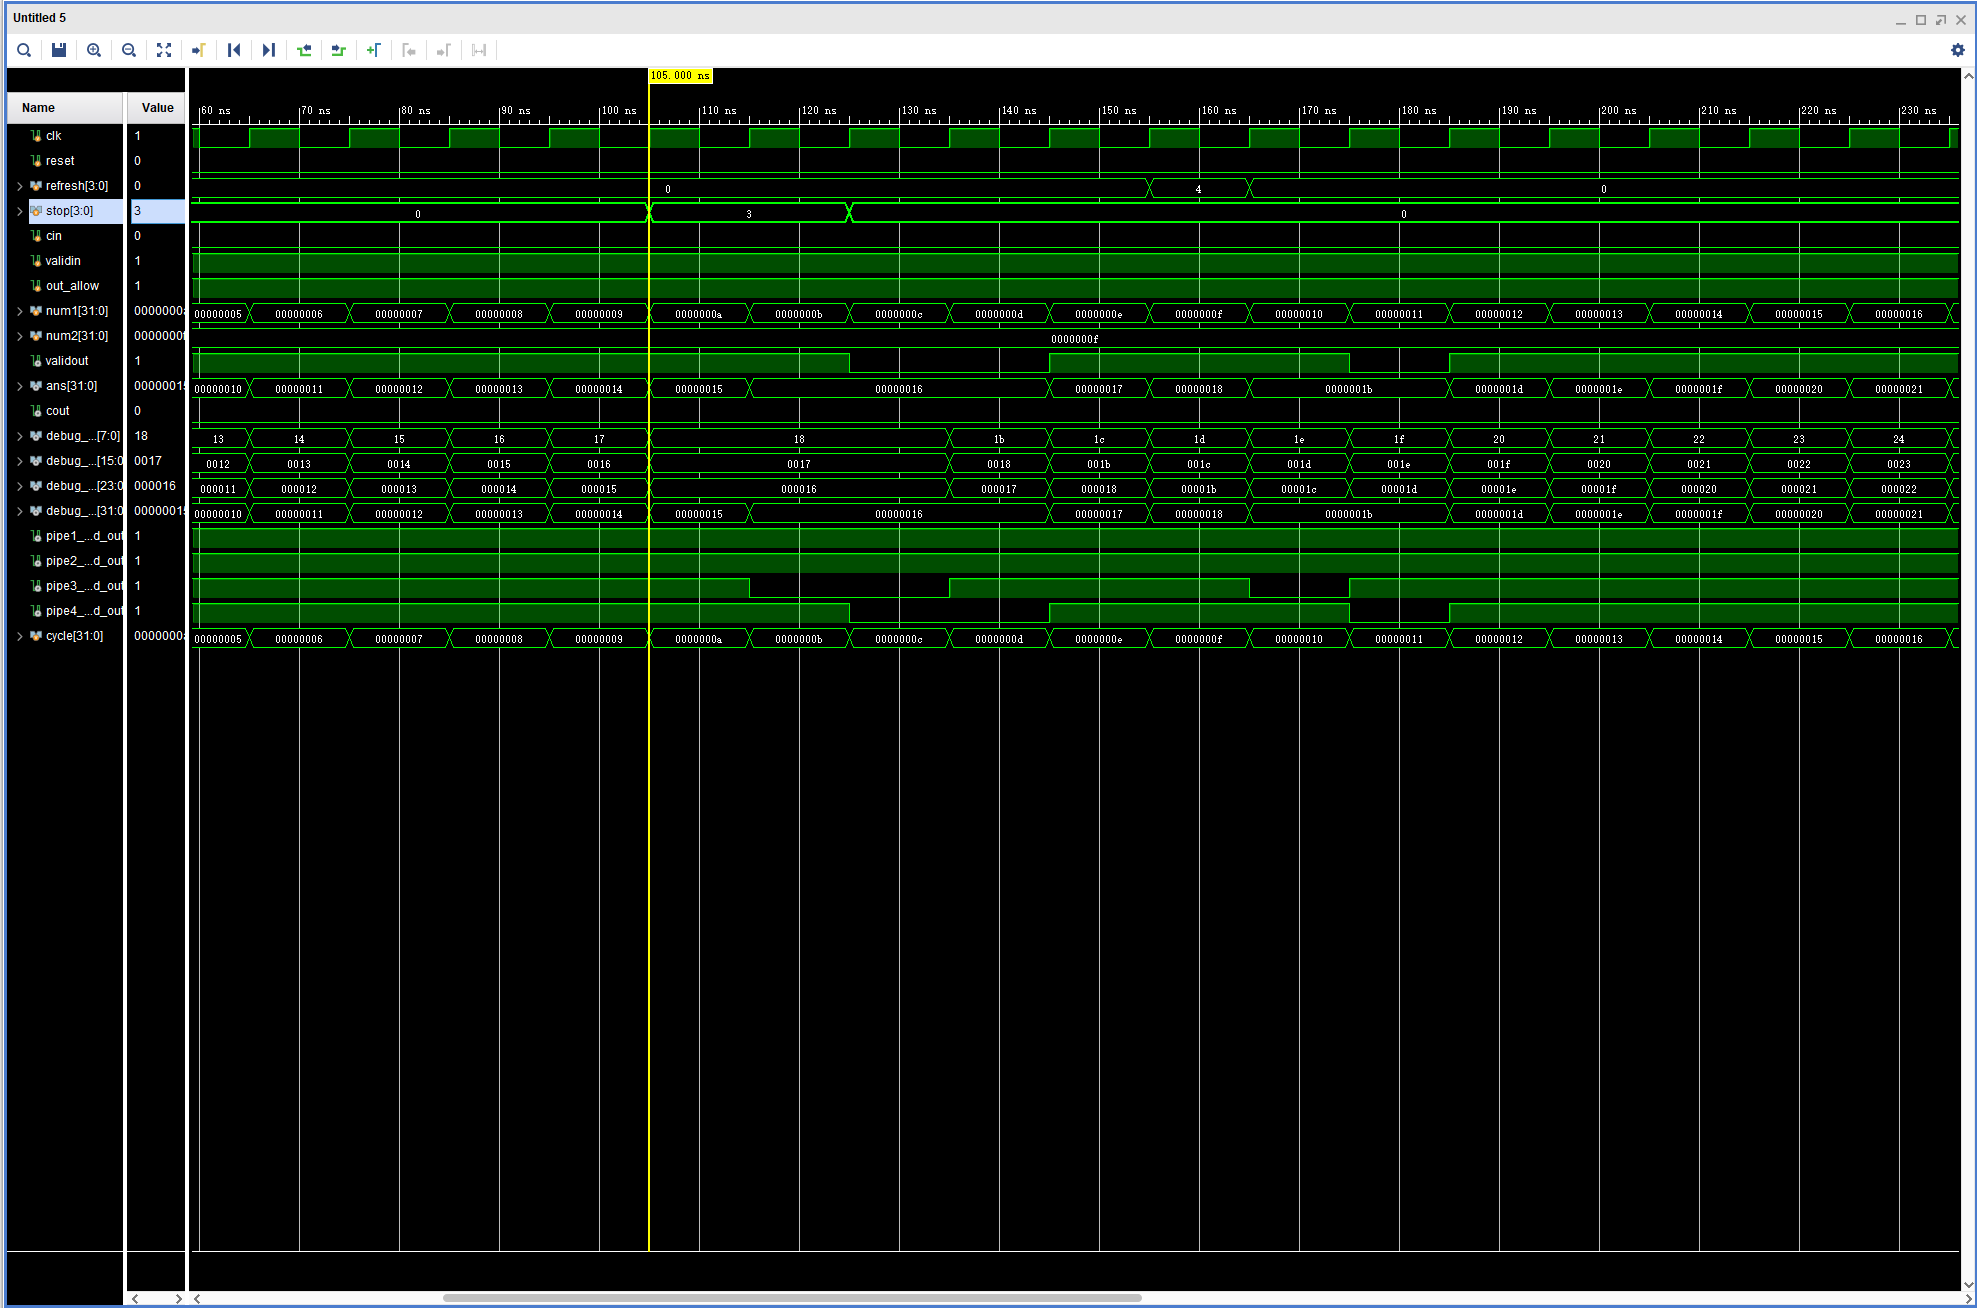
\includegraphics[width=0.5\textwidth]{image/177.png}
    \caption{流水线加法器暂停}
    \label{fig:my_label}
\end{figure}

\textbf{分析:}115ns 时,时钟上升沿,流水线加法器 stop 信号为 4'b0011,表示一二级流水线暂停。由图可知正常的结果延迟4周期再出现。而暂停后等待6周期才出现,表示成功暂停。并且此时0x00000016只在第一次出现的周期有效,后两个周期 validout 为 0 ,表示此结果无效。
\subsection{流水线刷新(清空)仿真图}
\begin{figure}[htbp]
    \centering
    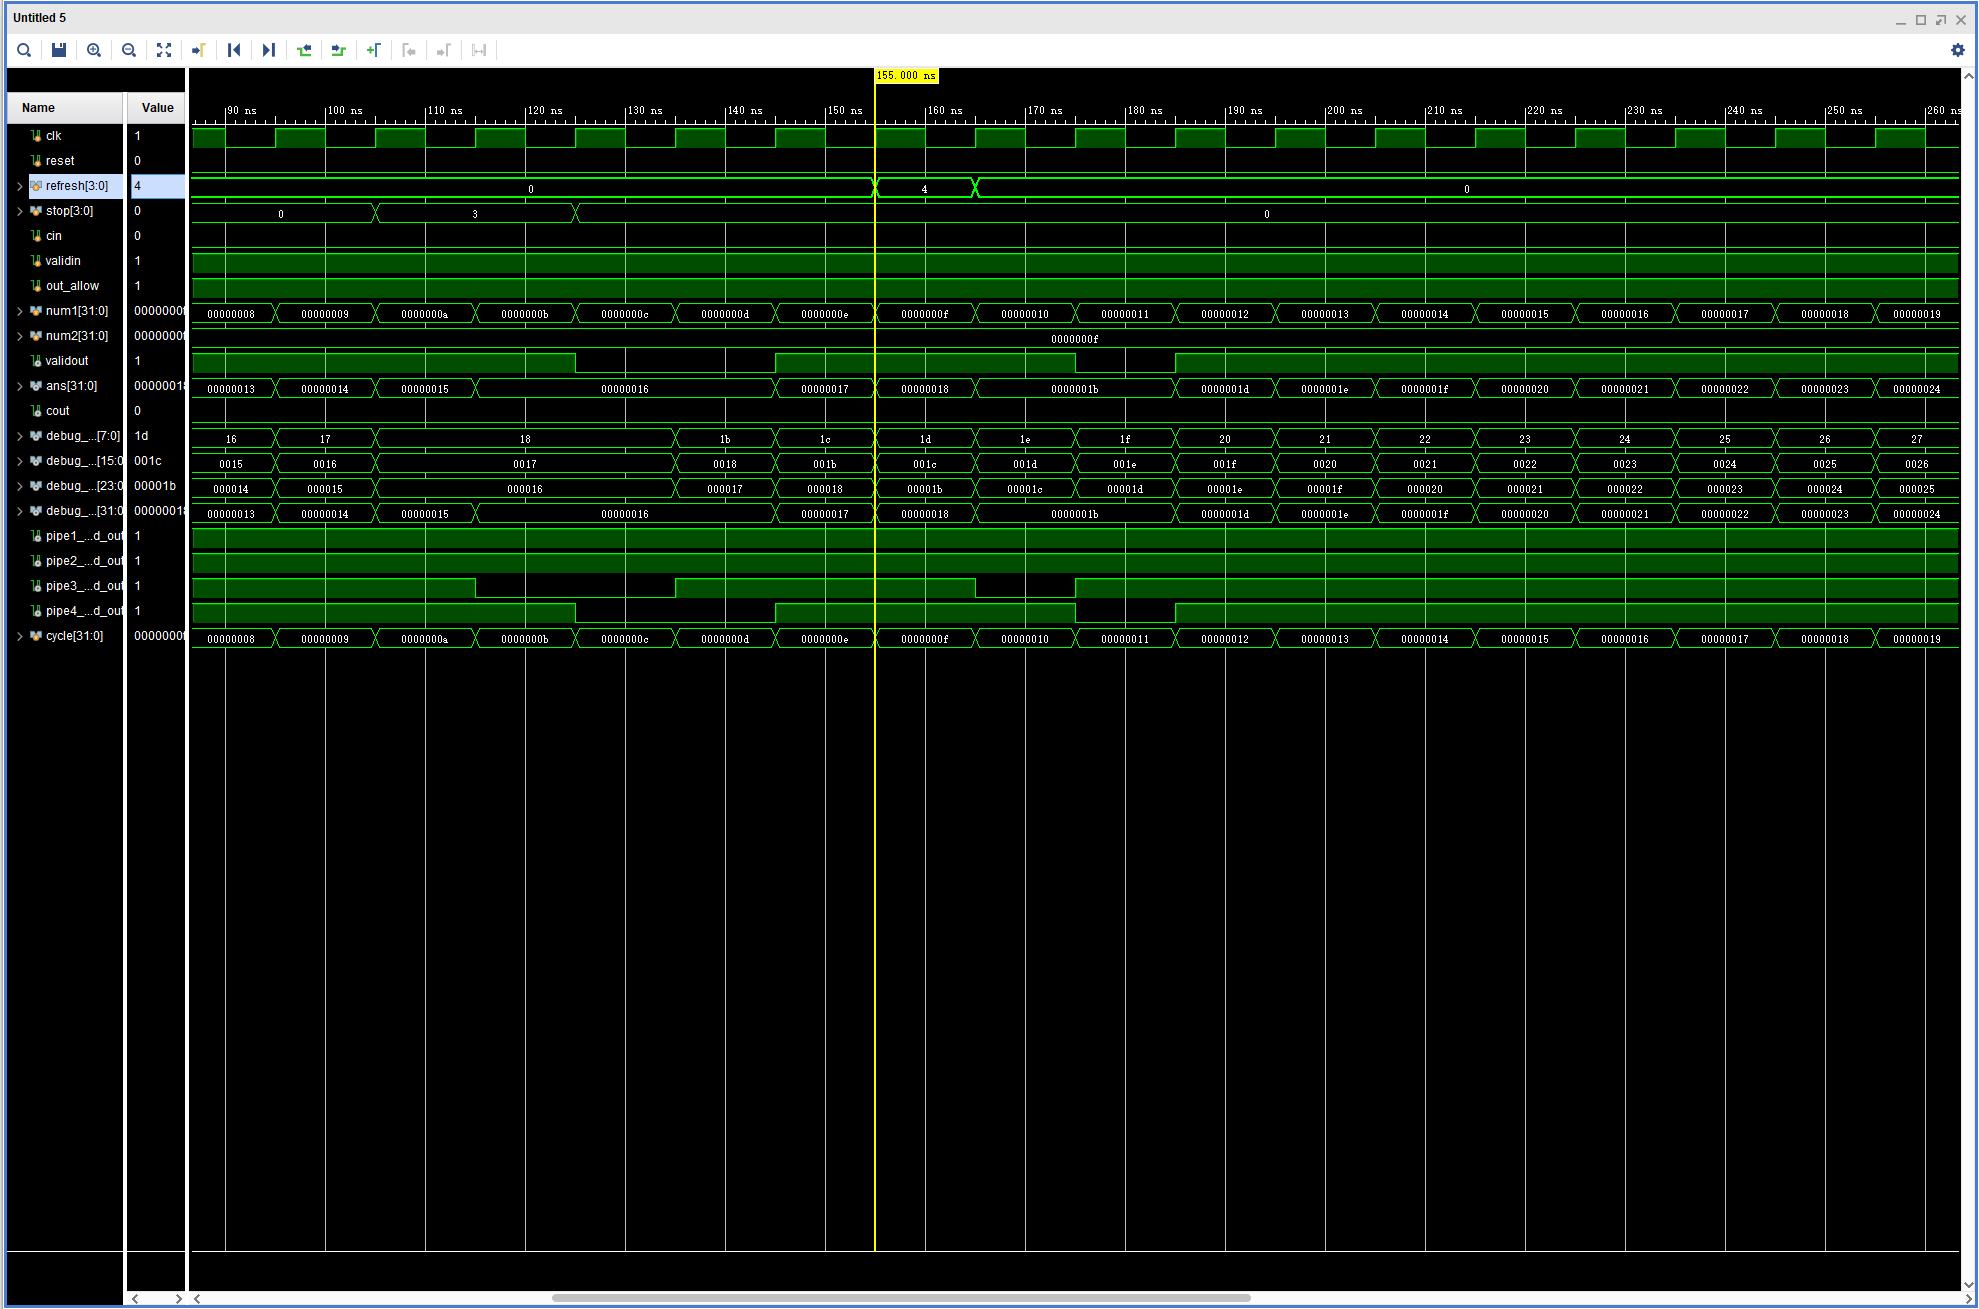
\includegraphics[width=0.5\textwidth]{image/33.png}
    \caption{流水线加法器清空}
    \label{fig:my_label}
\end{figure}
\textbf{分析:}165ns 时,时钟上升沿,流水线加法器 refresh 信号为 4'b0100,表示第三级流水线清空。由图可知, pipe3\_valid\_out 为 0,表示第三级流水线结果无效。并且本应该是0x0000001c的周期,结果为 0x0000001b,validout 信号为0,表示结果无效。由此可知成功刷新。